\section{Mail Filtering}

\paragraph{Simple Mail Transfer Protocol (SMTP)}
Protocol used to send and receive mail messages. For clients, SMTP is used to send emails to a mail server for relaying. To retrieve messages, IMAP (retrieve mail from a mail server) or POP3 are used (or others / proprietary protocols).

Boundary MTA use DNS to look up the MX record for the recipient's domain (after @). MX record contains name of target MTA

\begin{figure}[h]
	\centering
	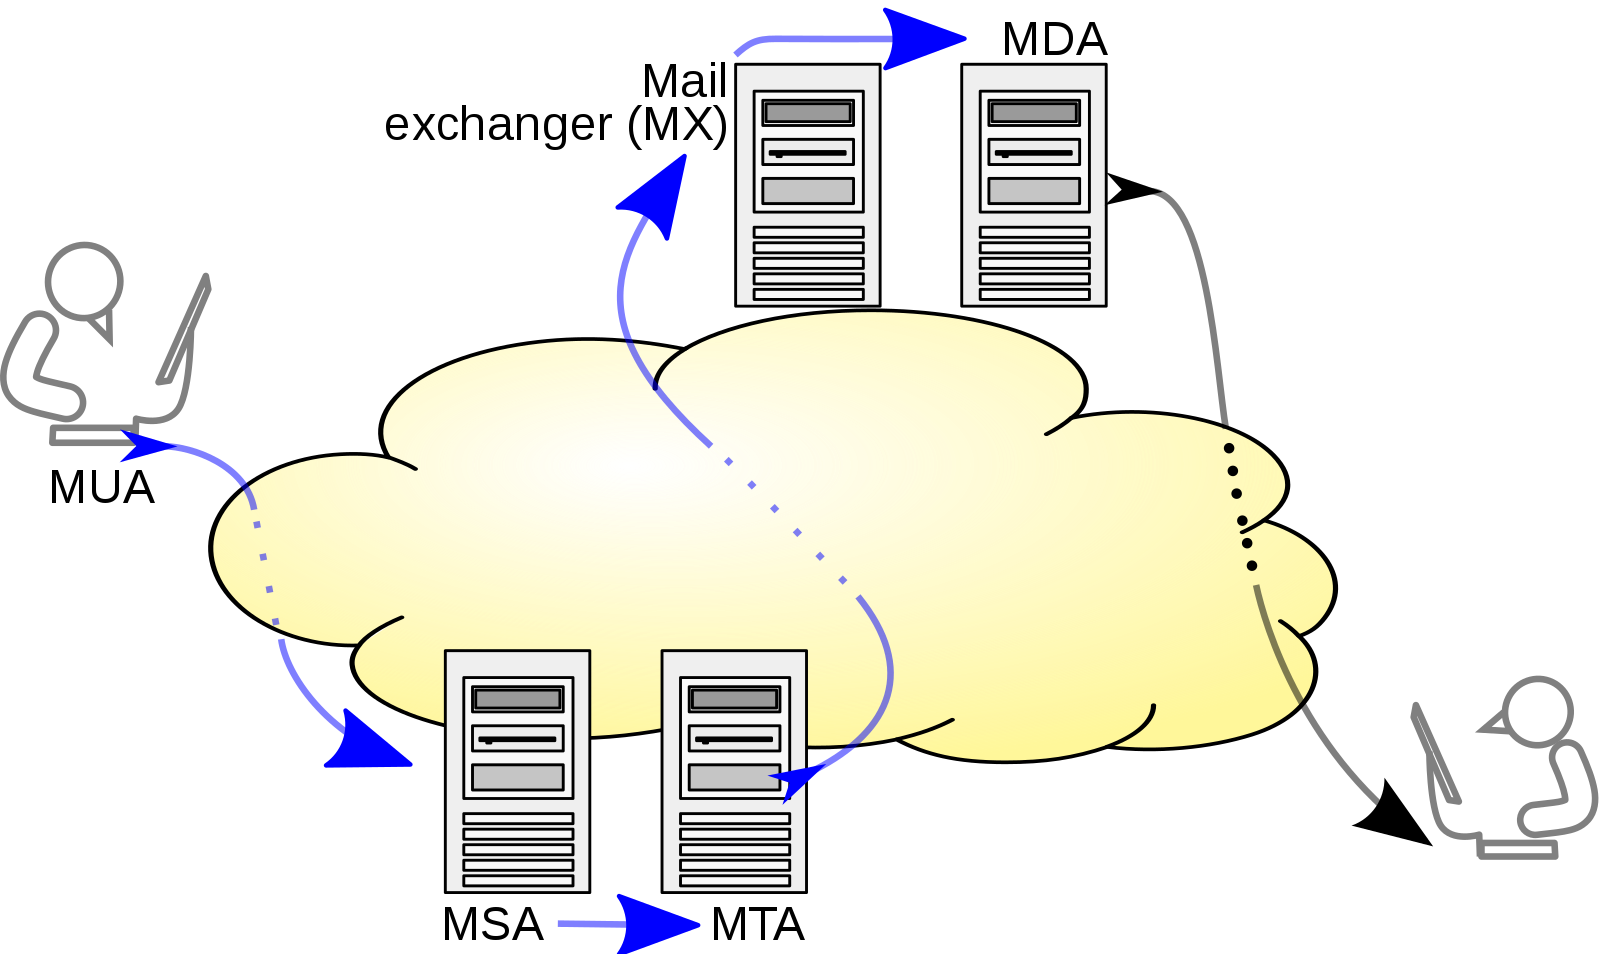
\includegraphics[scale=0.15]{images/916-smtp.png}
	\caption{Mail user agent sending an email to a mail submission agent, which in turn sends it to a mail transfer agent.}
	\label{fig:smtp}
\end{figure}

\begin{figure}[h]
	\centering
	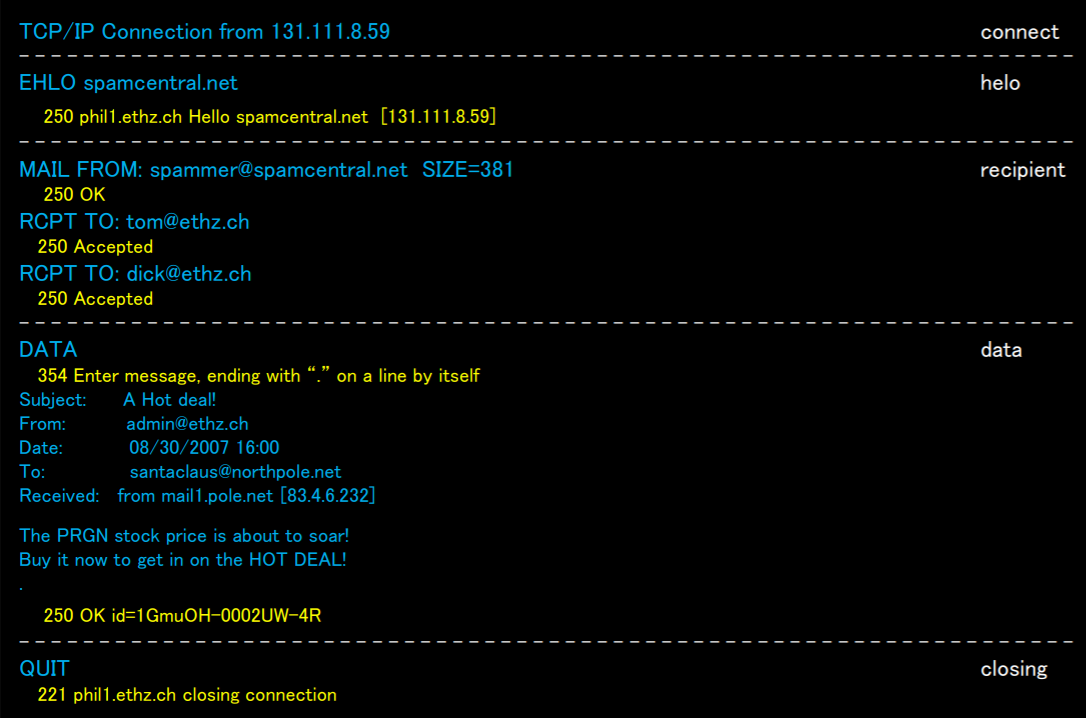
\includegraphics[scale=0.5]{images/916-session.PNG}
	\caption{Example of an SMPT message exchange. Note: actual sender and recipient does not match in message content.}
	\label{fig:session}
\end{figure}

\paragraph{Mail Filter}
There are several considerations when designing a mail filter:

\begin{itemize}
    \item Accept all and filter or already reject some during the SMTP session?
    \item Retrieve messages during a single SMTP session or multiple parallel ones?
    \item Filter only inbound mail or also outbound?
    \item Own DNS server for the filter?
    \item How to check valid recipient addresses? (local list, remote database, mail server, etc.)
    \item Will users have individual black- and whitelists?
    \item Will users have individual filtering preferences?
\end{itemize}